\documentclass{beamer}
\usetheme{CambridgeUS}


\title{Python Screenshot Project}
\subtitle{Automated Screenshot Taking and Markdown Generation}
\author{Anmol Narayan Smeet Singh Ankit Patel}
\institute{KIIT}
\date{\today}

\begin{document}

\begin{frame}
  \titlepage
\end{frame}

\begin{frame}{Project Overview}
  \begin{itemize}
    \item The goal of this project was to automate the process of taking screenshots while watching a video or in an online class.
    \item The project consists of three files: \texttt{screenshot.py} , \texttt{markdown.py} and \texttt{gallery.sh}.
    \item The first file takes screenshots at regular intervals and saves them in a new directory named \texttt{IMG}.
    \item The second file generates a Markdown file containing links to all the screenshots in the \texttt{IMG} directory.
    \item The project uses the Python imaging library (PIL) and the subprocess module in Python.
  \end{itemize}
\end{frame}

\begin{frame}{Screenshot.py}
  \begin{itemize}
    \item The \texttt{screenshot.py} file uses the PIL and numpy modules to capture and compare screenshots.
    \item It takes a command line argument that specifies the image change factor, which is the amount of change between the previous and current screenshots required to trigger a new screenshot.
    \item It saves each new screenshot in the \texttt{IMG} directory with a filename based on the current date and time.
  \end{itemize}

\end{frame}


\begin{frame}{Gallery.sh}
  \begin{itemize}
    \item The \texttt{gallery.sh} file generates a Markdown file that contains links to all the screenshots in the \texttt{IMG} directory.
    \item It uses a combination of Bash commands and Python code to create the Markdown file.
  \end{itemize}
\end{frame}

\begin{frame}{Demo}
  \begin{itemize}
    \item Here is a demo of the project in action.
    \item We will run the \texttt{screenshot.py} file with an image change factor of 0.05, which means that a new screenshot will be taken if there is a 5\% change between the previous and current screenshots.
    \item We will then run the \texttt{gallery.sh} file to generate the Markdown file.
  \end{itemize}

\end{frame}
\begin{frame}
	\frametitle{Running The bat file}
	\begin{center}
		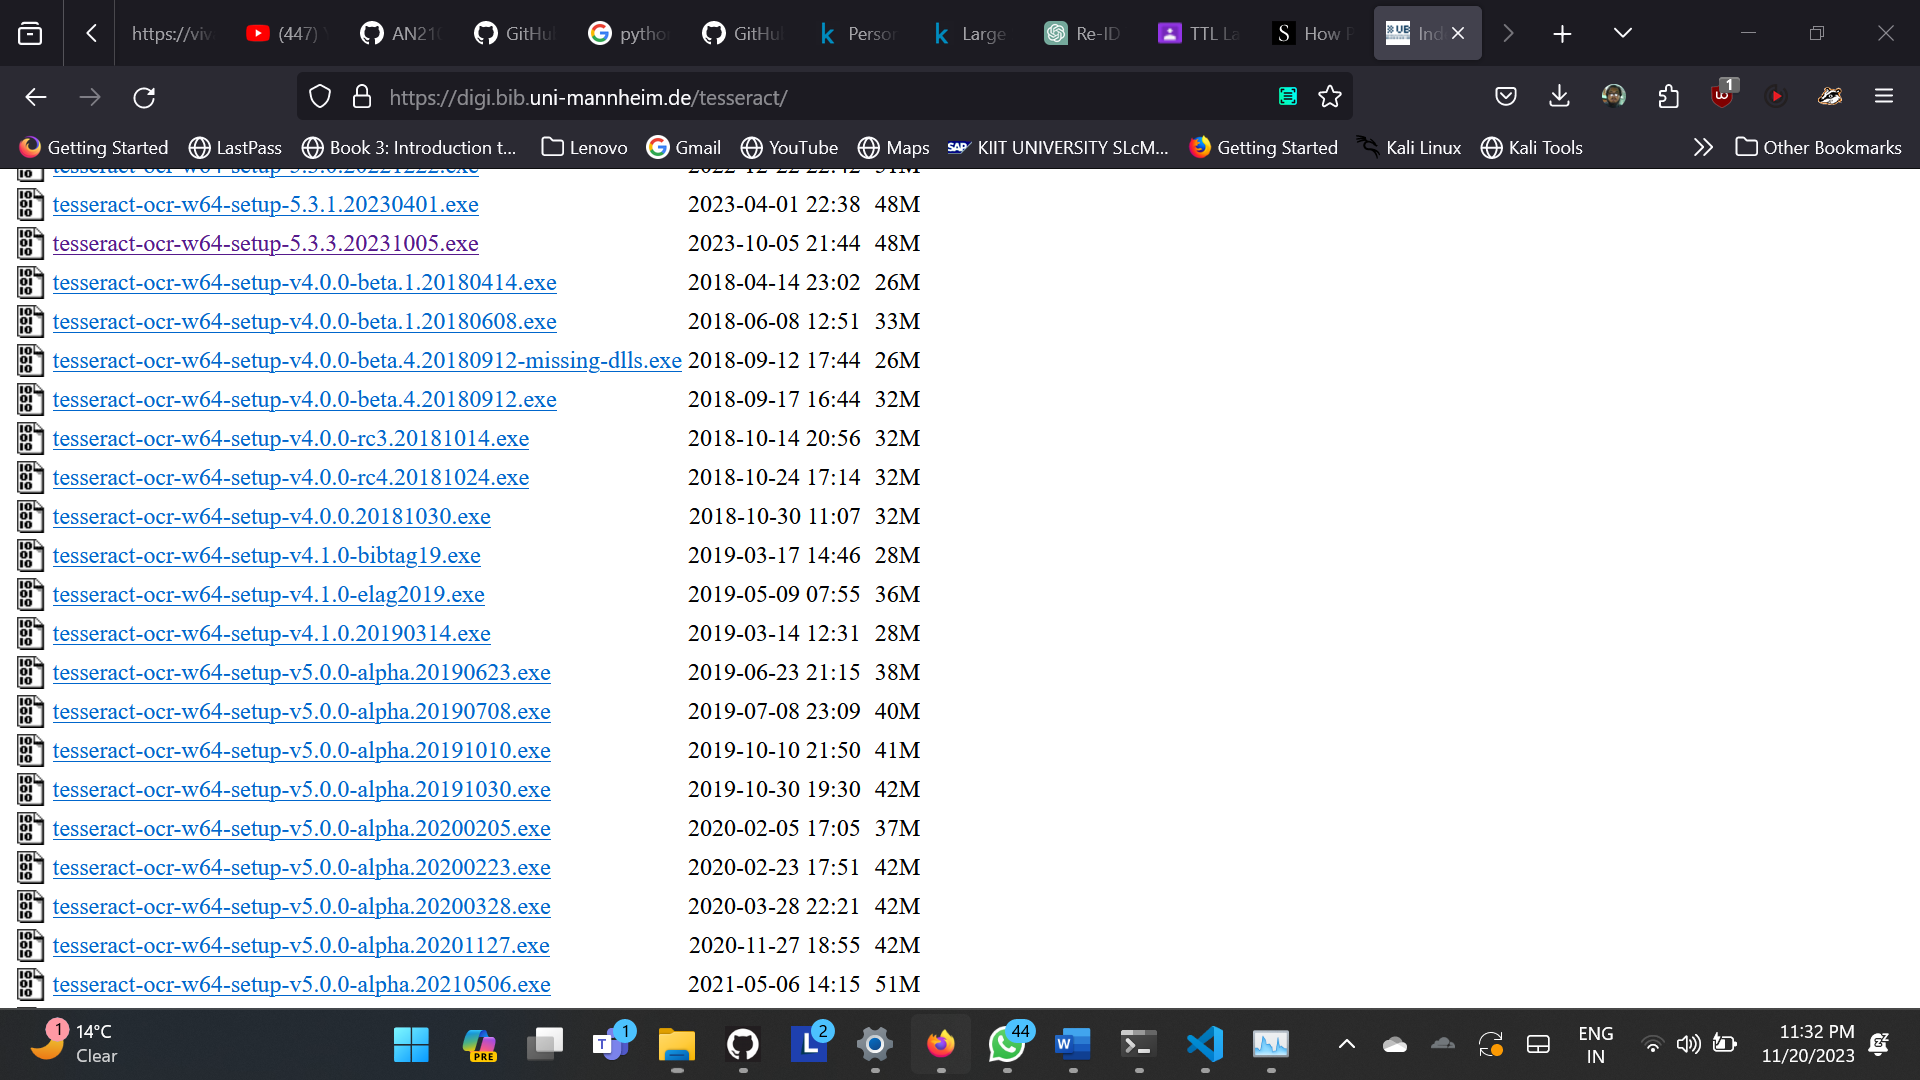
\includegraphics[width=0.9\linewidth]{1.png}
	\end{center}
\end{frame}
\begin{frame}
	\frametitle{Pressing Enter to exit}
	\begin{center}
		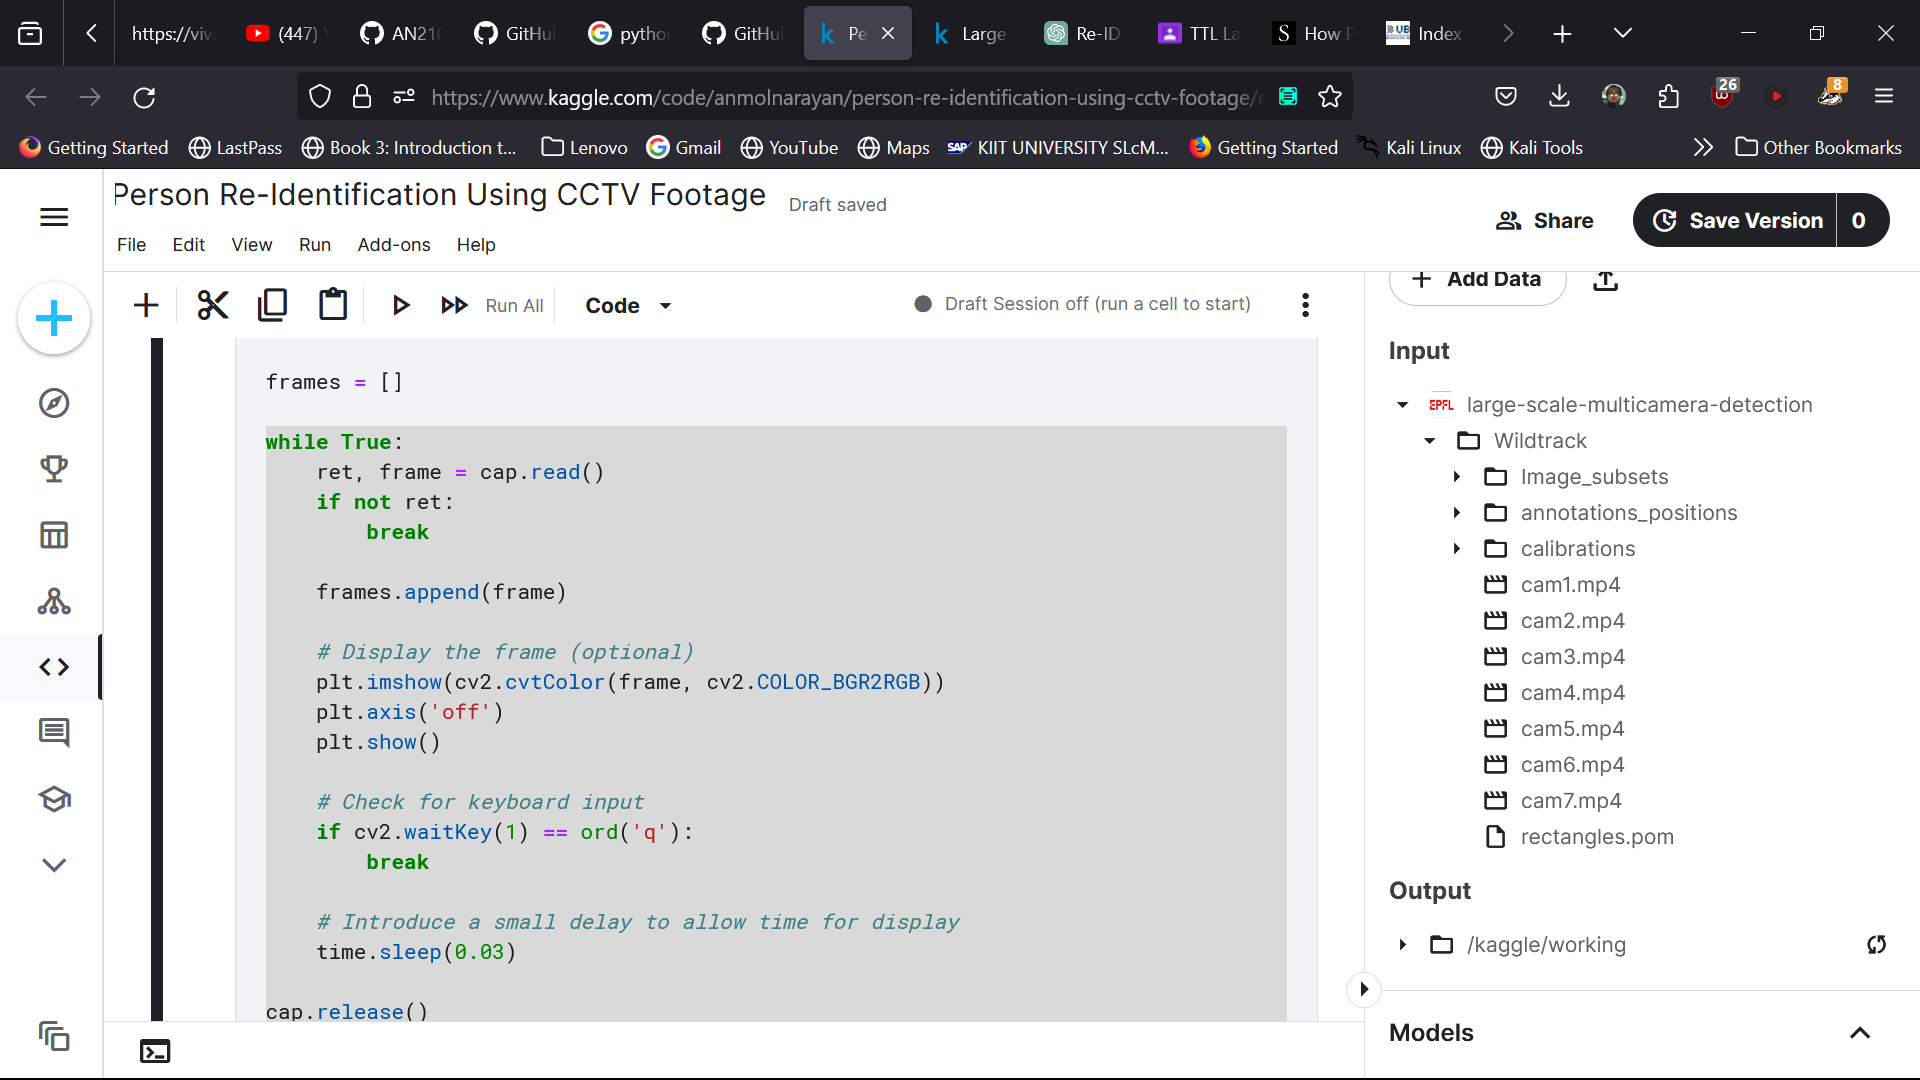
\includegraphics[width=0.9\linewidth]{2.png}
	\end{center}
\end{frame}
\begin{frame}
	\frametitle{The images stored in a folder}
	\begin{center}
		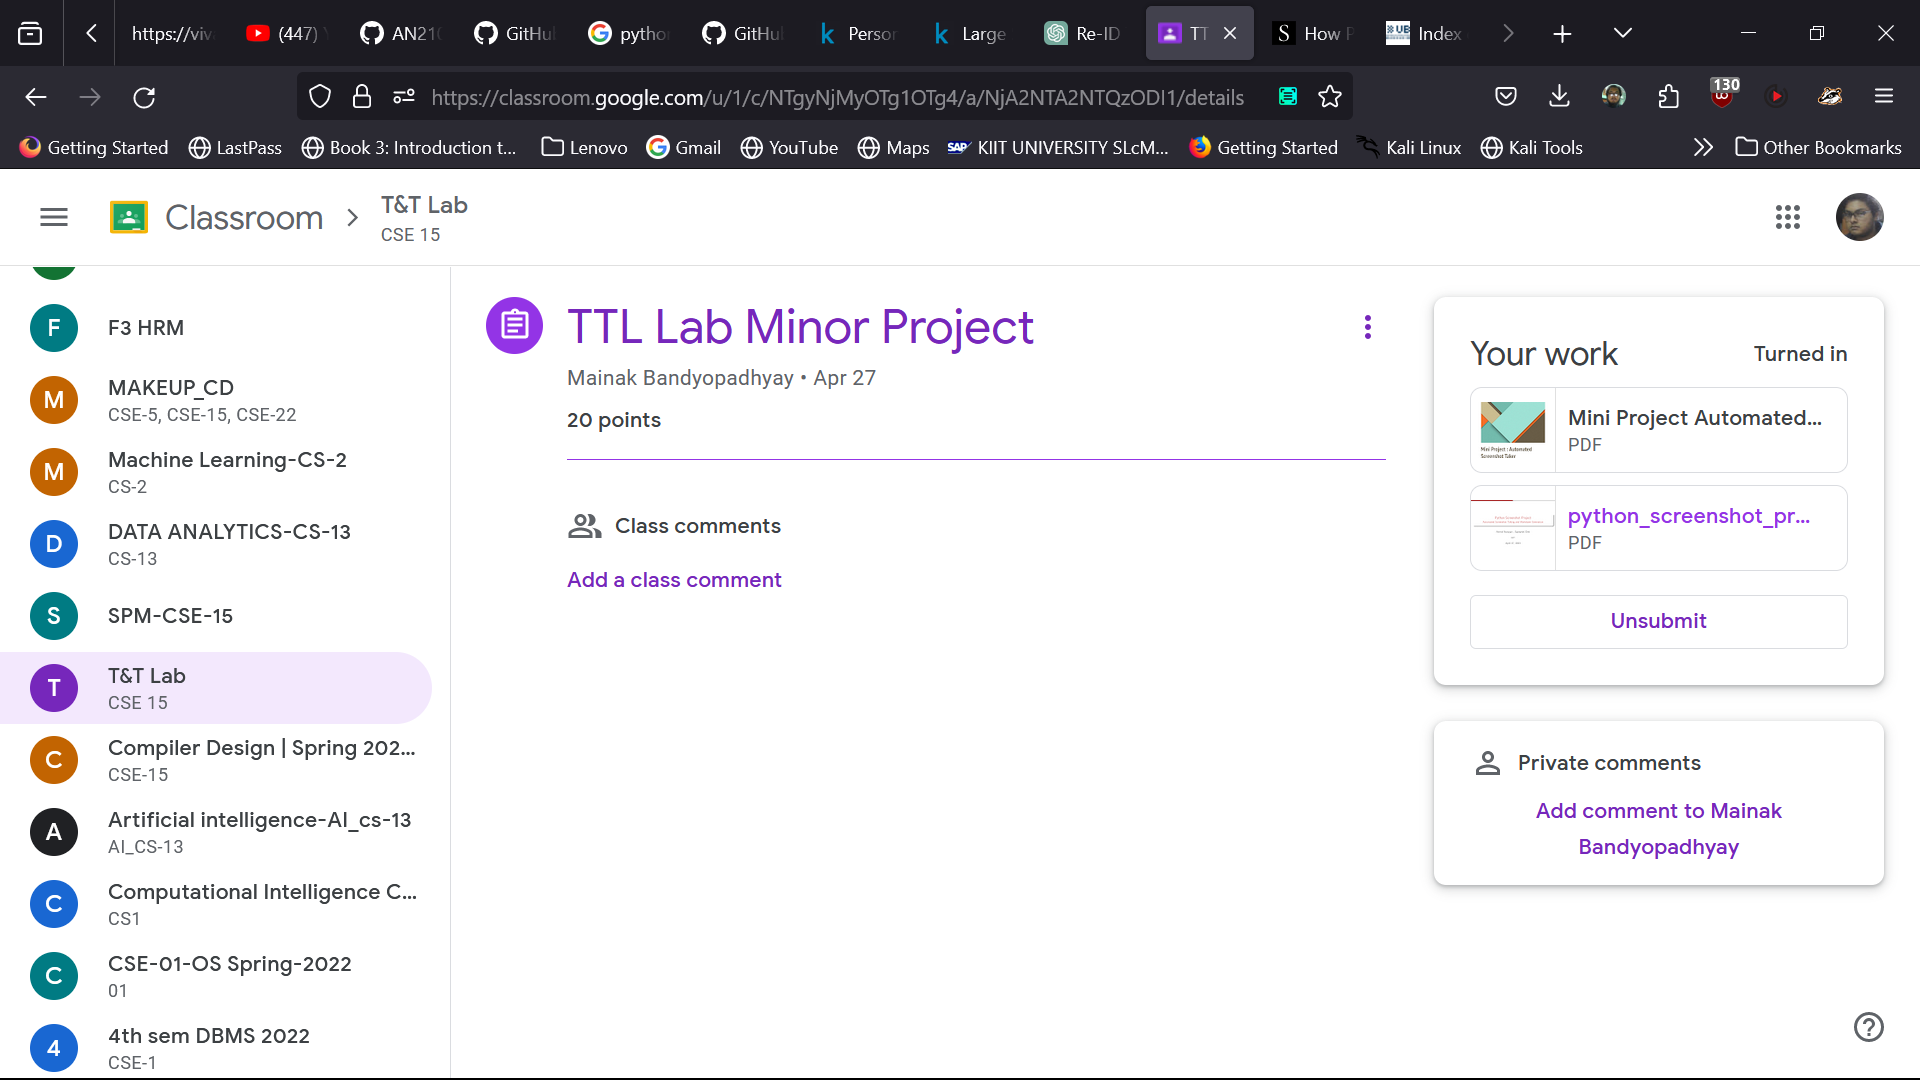
\includegraphics[width=0.9\linewidth]{3.png}
	\end{center}
\end{frame}
\begin{frame}
	\frametitle{Images linked together in markdown file}
	\begin{center}
		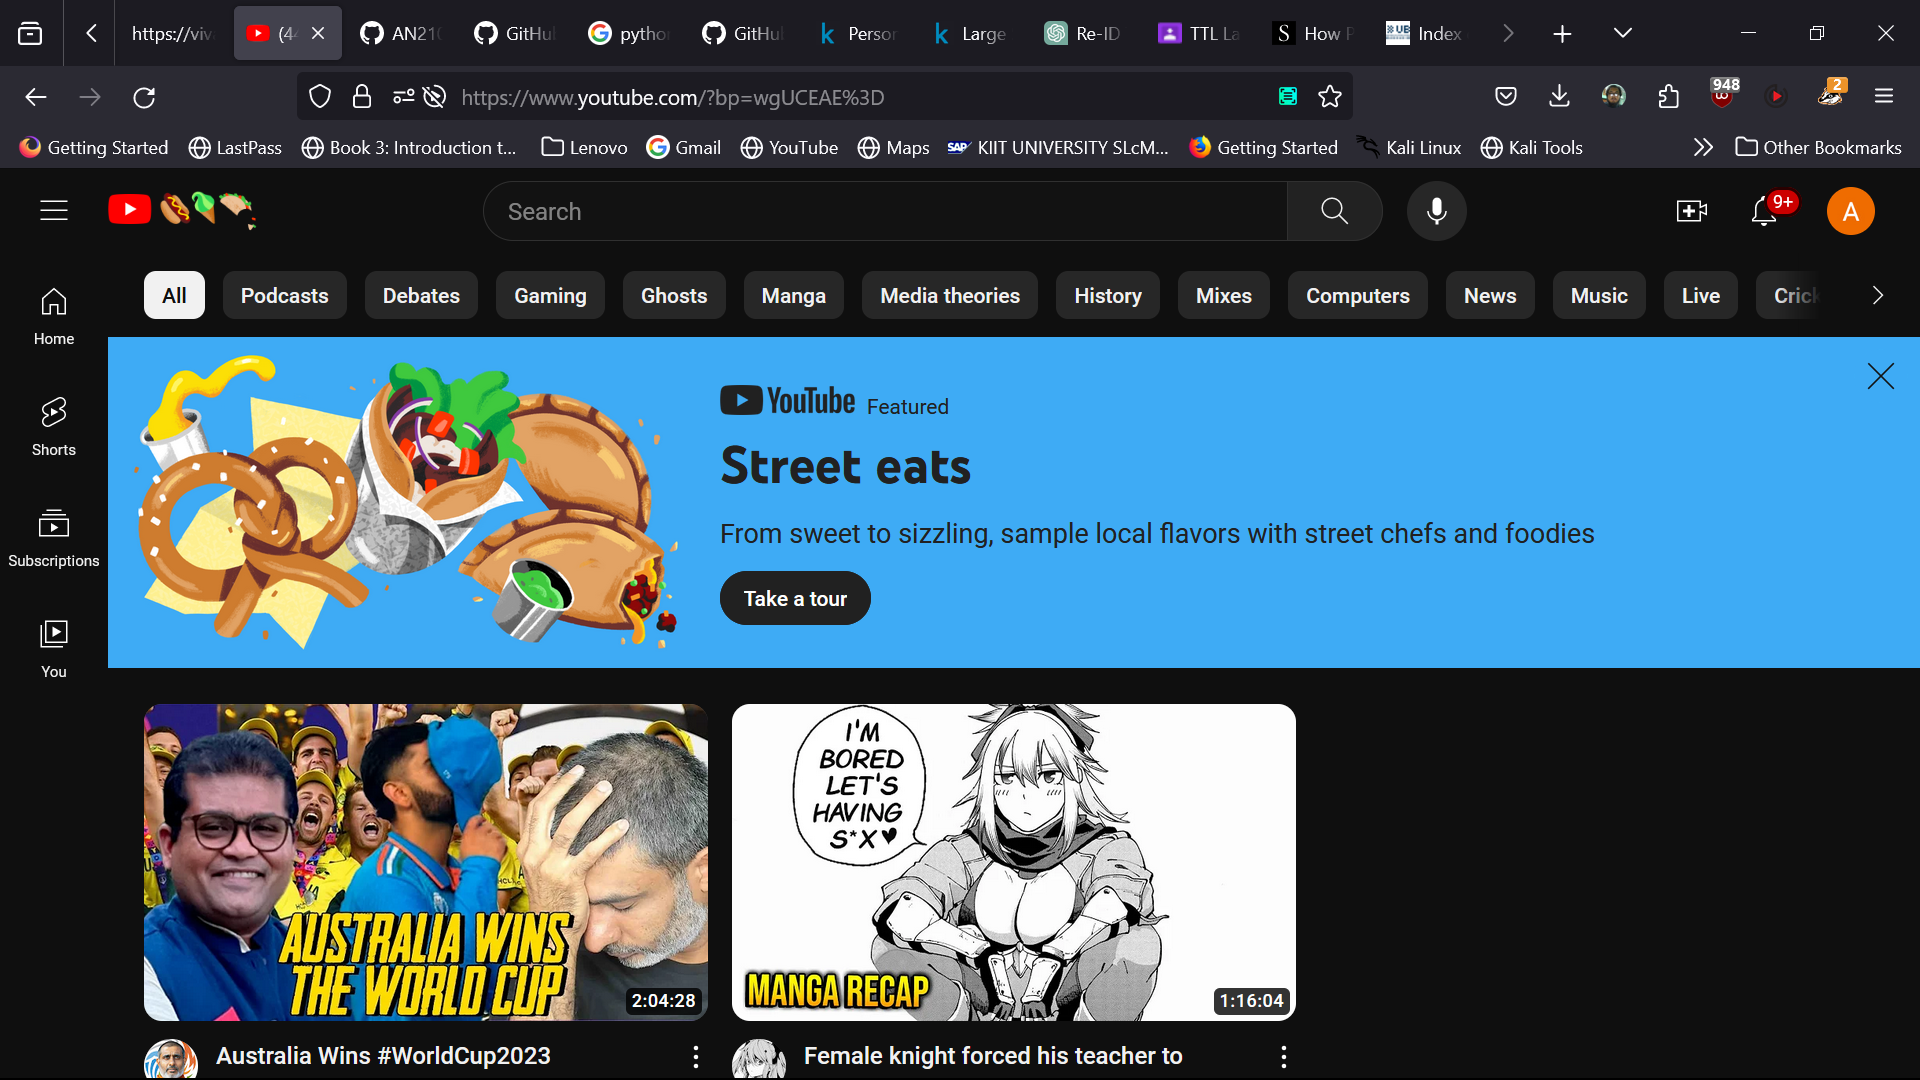
\includegraphics[width=0.9\linewidth]{4.png}
	\end{center}
\end{frame}

\begin{frame}{Tesseract OCR}
	\begin{itemize}
		\item Texts from the screenshots will be converted to text
		\item This feature help in converting the lecture videos content from presentation to simple texts
	\end{itemize}
\end{frame}
\begin{frame}{Conclusion}
  \begin{itemize}
    \item The Python screenshot project provides an easy and automated way to take screenshots while watching a video or in an online class.
    \item The project can be customized by changing the image change factor and the directory name for the screenshots.
    \item The project can be improved by adding more features, such as the ability to take screenshots only when a specific program is running or to automatically upload the screenshots to a cloud storage service.
  \end{itemize}
\end{frame}

\end{document}
